We discovered three main types of signals. First, strong signals emanate from switching voltage regulators and power filtering components at the specified switching frequency of the regulator (usually between 200 kHz and 500 kHz) or multiples of it (harmonics). These signals are modulated by variations in power consumption in the voltage regulator's load (the processor, memory or other system components), and they allow attackers to carry out the equivalent of power side-channel attacks from a distance without the need to place probes within the system. Voltage regulators for processor cores, the memory controller, and the DRAM memory itself often have different switching frequencies, giving the attacker component-by-component power consumption information. %Among voltage regulator designers, generated EM noise is a known problem and (cite saab here, explain doesn't demodulate).%we are not aware of any work that explores the implications of having the power consumption information embedded in the emanations caused by regulator switching .

Another type of signal is generated by periodic memory refreshes. This signal is amplitude-modulated by memory access activity, i.e. the attacker gets an at-a-distance readout of how often the memory is used. Unlike voltage regulators, which can be considered an external problem by processor/memory architects, these refresh-related signals are entirely caused by activity within the purview of memory controller designers and are likely to be completely eliminated by appropriate modifications to how memory refresh is carried out.

At higher frequencies, FASE discovers clock signals and their harmonics that are modulated by activity in the clock's domain. Because most clock and switching regulator harmonic frequencies are subject to electromagnetic interference (EMI) regulations~\cite{erickson_2001}, they are subjected to measures (such as spread-spectrum clocking) that spread the resulting EM emanations over a range of frequencies~\cite{hardin_1994}. In spite of this, FASE discovers such signals and provides insight into the nature of the activity that modulates them. In particular, we identify that DRAM clocks generate EM emanations which are modulated by DRAM activity. The systems tested generated weak spread-spectrum signals at CPU clock frequencies. Interestingly, we do not observe any variation in these signals in response to processor activity.

%%%%


We begin with Figure~\ref{spect_ldm}, which shows the FASE results for a recent desktop system with an Intel Core i7 processor, with the memory access modulation (LDM/LDL1) micro-benchmark. To emphasize the usefulness of FASE, we show a light gray outline of the actual recorded spectrum for one of the alternation frequencies. This spectrum is very noisy and crowded, especially in the long-wave (30-300 kHz) and AM radio (540-1600 kHz) bands, but FASE correctly indicates which signals are AM-modulated by the alternation activity. The thick vertical lines correspond to the frequency and magnitude of the modulated carrier signals automatically identified by FASE. Lines with the same color/pattern correspond to harmonics of the same frequency. A set of harmonics is likely caused by a periodic yet non-sinusoidal behavior within the system, and the magnitudes of the harmonics in a set give us important clues for identifying the source of that carrier signal. Therefore, after performing FASE it is useful to group the identified carriers into sets such that all the carriers within a set occur at frequencies which appear to be multiplies of one another.

The remainder of this section discusses how we used the information provided by FASE such as carrier frequency, harmonics, modulation depth, and modulation activity (e.g. on-chip activity or memory activity) to identify the sources of three types of carrier signals. In the systems not shown, similar types of signals were detected. 

\begin{figure}[tbh]
\centering
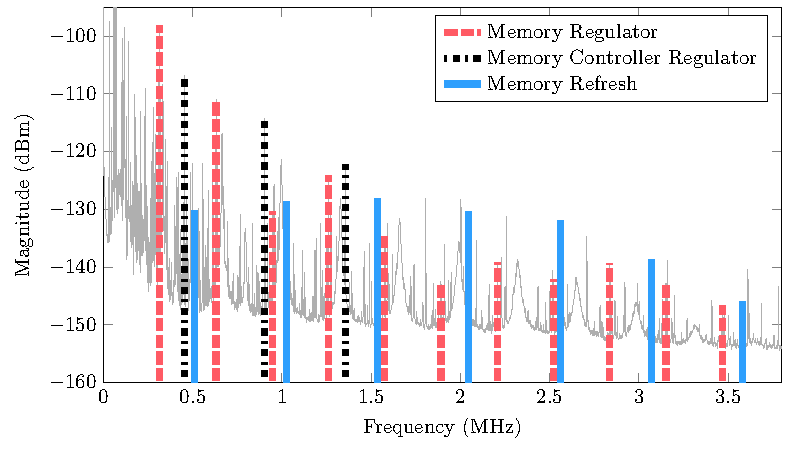
\includegraphics[trim=0.0in 0in 0in 0in,clip,width=5in]{../fase/Data/spect_ldm.pdf}%
\caption{FASE results for the Intel Core i7 desktop and main-memory (LDM/LDL1) modulating activity.}%
\label{spect_ldm}%
\end{figure}

\subsection{Switching Voltage Regulators}
\label{sec:regulators}

The set of carriers indicated by red dashed lines in Figure~\ref{spect_ldm} occurs at frequencies 315 kHz, 630 kHz, 945 kHz, etc., which are all multiples of 315 kHz. Because the even harmonics of this carrier are relatively strong we can conclude that these carriers are likely caused by some behavior that repeats at 315 kHz and has a small duty cycle. It is also helpful to look at each harmonic's shape in the spectrum. While this figure does not provide enough detail to see each harmonic's shape distinctly, the shape is very similar to that shown in Figure~\ref{core_reg_zoom} (this figure corresponds to a different regulator in the same system). The carrier's energy is spread around its central frequency by what looks like a Gaussian distribution. Clock signals for digital logic and I/O interfaces (such as memory) are tightly controlled but clocks generated by RC oscillators create carriers like the one in Figure~\ref{core_reg_zoom}.\footnote{This variation (called jitter or phase noise) is well studied because it impacts reliable communications and high frequency digital circuits~\cite{hajimiri_1998,trischitta_1989}.} 

Switching regulators often use RC oscillators. In computer systems, switching regulators convert the 12V to 24V PSU or battery voltage to 1V to 2V supplies used by processors and memory. The duty cycle of the regulator's switching signal is small when the ratio between the input and output voltage is large, which is consistent with the 315 kHz signal being related to a switching voltage regulator. We manually localized the source of the signal using an EM probe to determine where the 315 kHz EM signal was strongest in the system. We found that the signal was strongest near the high power MOSFET switches and power inductors that supply power to the main memory DIMMs. These switches were driven by a nearby switching voltage regulator IC and its switching frequency was 315 kHz, confirming our initial hypothesis. 

Once the source was found, the modulation mechanism was obvious: the regulator maintains the voltage supplied to the CPU by varying the duty cycle of the control signal of a switch between the 12V supply and the 1V output supply. For example, when DIMMs draw more current, the voltage at the regulator's output drops, so the regulator compensates by increasing the duty cycle of the switch, i.e. by connecting the 12V supply to its output for a longer fraction of the fixed 315 kHz period. When running the LDM/LDL1 microbenchmark, the DRAM regulator's duty cycle is increased during the DRAM accesses (LDM) and decreased during L1 cache hit activity (LDL1). Changing the duty cycle changes (modulates) the amplitude of all the signal's harmonics, so LDM/LDL1 activity modulates the emanated signal at the harmonics of the regulator's switching frequency.

\begin{figure*}[tb]
  \centering
    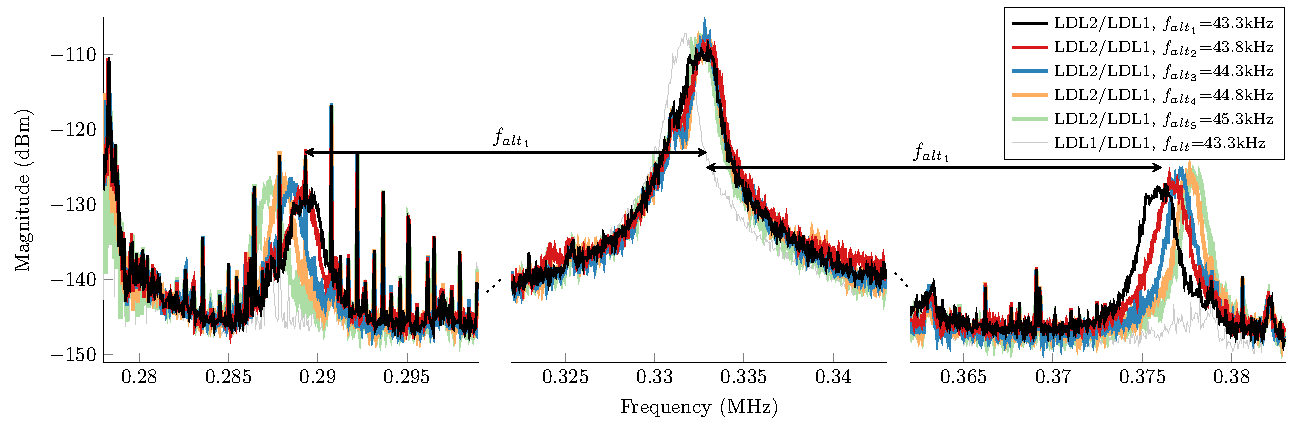
\includegraphics[width=\textwidth]{../fase/Data/core_reg_zoom.pdf}%
  \caption{A switching regulator related carrier at $f_c$ and its right and left side-bands generated by on-chip activity.}%
  \label{core_reg_zoom}%
\end{figure*}

\begin{figure}[thb]
\centering
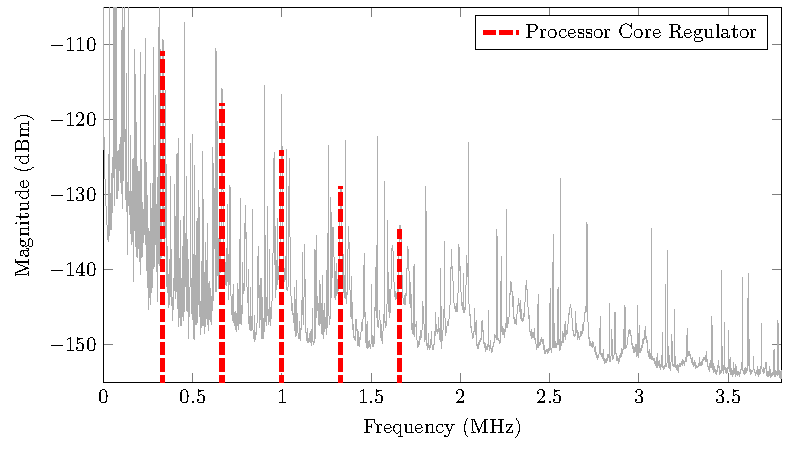
\includegraphics[trim=0.0in 0in 0in 0in,clip,width=5in]{../fase/Data/spect_ldl2.pdf}
\caption{FASE results for Intel Core i7 desktop and L2 cache (LDL2/LDL1) modulating activity.}
\label{spect_ldl2}
\end{figure}

Carrier signals indicated by black dash-dot lines in Figure~\ref{spect_ldm} are also caused by another voltage regulator. This regulator powers the on-chip memory interface (the chip has separate power supplies for its cores and its memory interface). Figure~\ref{spect_ldl2} shows the spectrum for heavy on-chip alternation activity (LDL2/LDL1). Only one type of carrier was found to be modulated in this case -- the signal that corresponds to the switching regulator for the CPU cores. Figure~\ref{core_reg_zoom} shows one of the harmonics of this signal in greater detail. We confirmed the origin of both memory interface and core regulator signals through the same near-field localization process. Interestingly, the prominent Gaussian-like shapes of the core regulator's signal are also visible in Figure~\ref{spect_ldm} but were not reported by FASE because they were not significantly modulated by the LDM/LDL1 alternation. This again illustrates that strong signals are not necessarily modulated by the activity under observation.

In many recent processors, the core CPU voltage is adjusted dynamically, while many on-chip cache and memory interface designs require fixed voltage supplies. Therefore, some processors require separate voltage regulators for the CPU and cache. As we have demonstrated, a regulator's carrier is modulated by the activity in the circuit it powers, so an attacker can distinguish cache and CPU activity by demodulating each regulator's carrier separately. Also, when separate dynamic voltage scaling is used for each CPU core, each core requires a separate regulator. When such regulator switching frequencies are not identical, attackers might be able to remotely receive a separate power consumption readout for each core, allowing attackers to remotely perform a separate power analysis attack for each core.

Finally, we note that the emerging use of in-package/on-chip regulators for processors affects regulator-related EM information leakage in new and interesting ways. On-chip linear regulators~\cite{wang_2013} do not produce modulated emanations because they have no switching frequencies to modulate. The integration of switching regulators has a more complex impact. Each integrated regulator supplies a smaller part of the chip, so the switching currents are lower and follow shorter paths, reducing emanations. However, integrated switching regulators use higher switching frequencies (e.g. 140 MHz in \cite{burton_2014}) resulting in stronger emanations. Higher switching frequencies also allow faster reactions to changes in the output voltage providing attackers with a higher bandwidth readout of power consumption.

\subsection{Memory Refresh}

The modulated carrier shown in Figure~\ref{spect_ldm} as solid blue lines has harmonics at frequencies of 512 kHz, 1024 kHz, etc. This signal did not match any previously known mechanisms that can cause EM emanations. It has a very stable frequency, indicating it was likely generated by logic that is clocked with a crystal-oscillator derived clock. Its harmonics are all of similar strength, indicating an extremely small ($<$5\%) duty cycle. Localization showed that this signal was strongest near the memory DIMMs. Additional experiments showed that the carrier signal is strongest when there is no memory activity and weakest when we generate continuous memory activity. 

This is unusual -- if this signal is caused by memory activity, we would expect it to get stronger with more activity. Further measurements with small probes close to the memory revealed many additional harmonics with a greatest common divisor of 128 kHz, not 512 kHz. This was the key clue in solving the puzzle, because 128 kHz corresponds to a period of 7.8 $\mu$s, the maximum allowable average time between refresh commands for recent DRAM standards such as DDR3.

While it would be difficult to conclusively prove that this signal is generated by memory refresh activity, the evidence strongly suggests it is. The duty cycle of the memory refresh activity is very low ($<$ 3\%) because each refresh command only lasts approximately 200 ns and occurs every 7.8 $\mu$s. The refresh timing is derived from the memory controller clock, which is crystal-derived. While DRAM standards specify that the average time between refresh commands must not exceed 7.8 $\mu$s, the memory controller has some control over the timing of the refresh commands. For example, the memory controller could postpone sending refresh commands during a 40 $\mu$s period of intense memory activity, and then ``catch up'' when memory has some idle time. This explains the strangest observation about this signal, which was that it weakens (instead of getting stronger) as memory activity increases. When the memory is inactive, the memory controller simply sends memory refresh commands at regular intervals, resulting in the strongest signal at that interval's frequency. As memory activity increases, the memory accesses increasingly interfere with the timing of the refresh commands, causing refreshes to be delayed and disrupting their periodicity (thus spreading their emanated energy across a much larger frequency range and causing the signals at 128 kHz, 256 kHz, etc. to weaken). Although the first harmonic of this signal is weaker than regulator-related signals, note that memory refresh produces many modulated harmonics and that attackers can potentially correlate them to dramatically improve their detection of this signal and its signal-to-noise ratio. It is also worth noting that since refresh timing is dictated by a standard, refresh carrier signals are present at roughly the same frequencies on all the systems we tested, which could simplify the exploitation of this leakage. This potential problem likely has an easy fix: randomizing the issue of memory refresh commands would be compatible with existing DRAM standards and would greatly reduce the modulation of refresh activity.

\subsection{DRAM Memory Clock}
%

\begin{figure}[t]
\centering
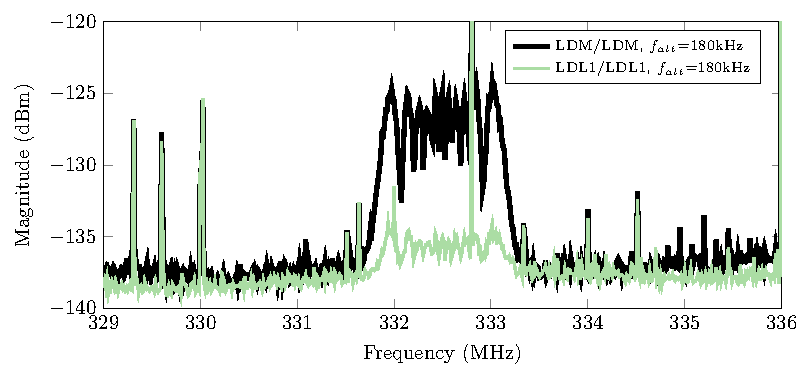
\includegraphics[trim=0.1in 0.10in 0.1in 0.09in,clip,width=5in]{../fase/Data/lx61_mem_ssc_a.pdf}
\caption{DRAM clock spectrum with 0\% (LDL1/LDL1) and 100\% (LDM/LDM) memory activity.}
\label{lx61_mem_ssc_a}
\end{figure}

\begin{figure}[b]
\centering
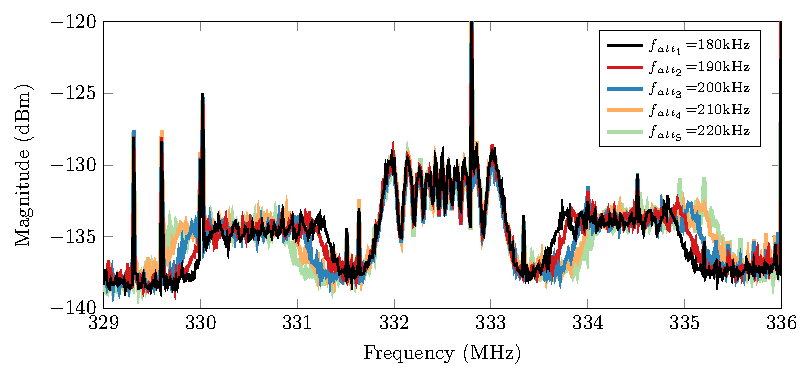
\includegraphics[trim=0.1in 0.10in 0.1in 0.09in,clip,width=5in]{../fase/Data/lx61_mem_ssc_b.pdf}%
\caption{DRAM clock spectrum with 50\% (LDM/LDL1) memory activity.}%
\label{lx61_mem_ssc_b}%
\end{figure}
Above 30 MHz, electromagnetic compatibility (EMC) standards limit the allowable level of EM emanations from consumer devices such as computers. Many periodic signals such as high frequency processor and memory clocks are strong enough to violate these limits, so alleviation techniques for these clock signals have been developed. EMC requirements specify the maximum magnitude for emissions at any particular frequency, and a popular technique (called spread spectrum clocking) varies the clock frequency periodically, spreading the emitted energy across a range of frequencies (instead of emanating it all at one frequency). For example, a 333 MHz memory clock might be swept back and forth between 332 MHz and 333 MHz over a period of 100 $\mu$s, producing a spectrum similar to %Figure~\ref{lx61_mem_ssc}\textcolor{red}{A}. 
Figure~\ref{lx61_mem_ssc_a}. While such techniques facilitate compliance, the signals are only weaker in an averaged sense: attackers can still track the carrier and use the full power of the signal after demodulation. Such ``carrier tracking'' techniques have already been developed in telecommunications to allow reception of radio signals transmitted using this technique~\cite{chung_1993}. Therefore, predictable spread-spectrum clocking does not mitigate information leakage, but it does create interesting problems for discovering such modulated carriers through manual analysis of the spectrum. The shape of the carrier and its side-bands is less recognizable, and the carrier and its side-band signals are likely to overlap significantly when using modulation activity that is not carefully chosen. 

To allow FASE to successfully detect modulated spread-spectrum clocks, it is best to set $f_{alt}$ large enough to move the side-band signals outside of the carrier's own spectrum. Figure~\ref{lx61_mem_ssc_b} shows the effect of modulating the clock signal at several such alternation frequencies.
%

\subsection{Testing the Laptop Systems}

We tested three laptop systems: one based on an Intel Core 2 Duo processor from 2010, one based on AMD Turion X2 from 2007, and one based on Intel Pentium 3M from 2002. In all three systems, FASE finds the same types of carriers we already reported: regulator-related signals, signals caused by memory refresh, and DRAM clock signals. For example, Figure~\ref{hpamd_spect_ldm} shows the modulated carrier signals found for the AMD Turion X2 system with LDM/LDL1 alternation of activity. Interestingly, the memory refresh carrier for the AMD Turion X2 laptop is at 132 kHz instead of 128 kHz as observed in all three other systems. We also confirmed a memory regulator carrier and while the two signals shown as ``unidentified'' appear to be caused by regulators, we did not confirm their sources because the laptop is very compact and taking it apart to perform localization may damage the system.

\begin{figure}[htb]
\centering
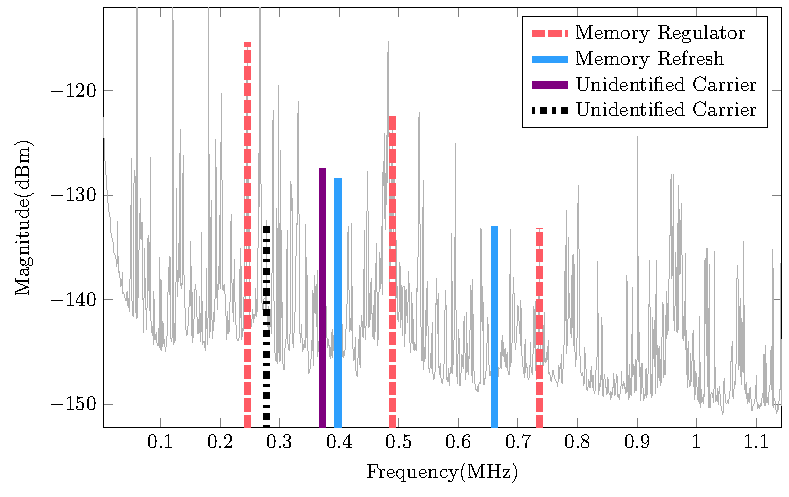
\includegraphics[trim=0.0in 0in 0in 0in,clip,width=5in]{../fase/Data/hpamd_spect_ldm.pdf}%
\caption{FASE results for the AMD Turion X2 laptop and main-memory (LDM/LDL1) modulating activity.}%
\label{hpamd_spect_ldm}
\end{figure}

The AMD system was the only system confirmed to have an activity-modulated carrier that is not reported by FASE. This carrier was emanated by the voltage regulator circuitry for the processor cores, and was \emph{frequency}-modulated (we confirmed this with a spectrogram of the modulation). Therefore FASE correctly does not report it. This particular regulator keeps the input-to-output switch turned on for a fixed amount of time during its switching cycle, but changes the duration of the switching cycle (i.e. its switching frequency) to increase/decrease its duty cycle. In principle, signals that are frequency-modulated by system activity should be possible to identify by a FASE-like approach based on spectral properties of FM-modulated signals. 

%We leave the design of such FM-seeking approaches for future work.
